\documentclass[11pt,a4paper]{article}
\usepackage[T1]{fontenc}
\usepackage{lmodern,microtype,amsmath,amssymb,amsthm,mathtools}
\usepackage[margin=25mm]{geometry}
\usepackage{booktabs,graphicx,tabularx,array}
\usepackage[section]{placeins}
\usepackage{xcolor,xurl}
\usepackage[colorlinks=true,allcolors=blue]{hyperref}
\newtheorem{theorem}{Theorem}[section]
\newtheorem{proposition}[theorem]{Proposition}
\newtheorem{lemma}[theorem]{Lemma}
\DeclareMathOperator{\sech}{sech}
\DeclareMathOperator{\artanh}{artanh}
\DeclareMathOperator{\tr}{tr}
\allowdisplaybreaks[1]
\setlength{\emergencystretch}{2em}
\hypersetup{pdfauthor={Muacca},pdftitle={Adiabatic Endpoint Polarizations for Dirac Fields on Anisotropic Compact Cosmologies: Fock Implementability and Excitation Energy},pdfsubject={Version 1, first release 2026-11-22}}
\title{Adiabatic Endpoint Polarizations for Dirac Fields on Anisotropic Compact Cosmologies: Fock Implementability and Excitation Energy}
\author{Muacca}
\date{Version 1\\First release: 2026-11-22}
\begin{document}
\maketitle
\begin{abstract}
We propagate an external massless Dirac field between two round ends of an exact biaxial three-sphere cosmology. The instantaneous endpoint splittings give non-Hilbert--Schmidt mixing. With first-order adiabatic endpoint polarizations the expected particle and hole counts are positive and finite, while the sum of their absolute physical endpoint energies weighted by occupation diverges logarithmically in the shell cutoff. Second order makes this energy finite. A uniform two-level estimate gives convergence up to the magnetic lattice edge, and a discrete phase estimate on an interior band supplies the logarithmic lower bound. Interval integration of 551 magnetic pairs plus an analytic ultraviolet tail bounds the two finite counts and the second-order energy. On two intervals of an expanding compact Nil geometry, a separate two-index summation proves failure of instantaneous implementability and convergence at first order. The observables use specified endpoint projections and an external field on each prescribed history.
\end{abstract}
\section{The endpoint question}\label{sec:01}
Consider a compact universe with a round three-sphere at each of two times. The intrinsic metrics at the ends can agree while the shape velocities have opposite signs. A massless spinor then sees equal instantaneous energy splittings at the two ends, but their eigenspaces turn through the interval. We ask two questions about the transported vacuum. Is the off-diagonal part of the one-particle evolution Hilbert--Schmidt, so that a Fock-space evolution exists? If it does, does weighting each excited particle and hole by its endpoint energy still give a finite sum?

We answer both for one exact nonround return of the fixed-charge Einstein--scalar system. On this geometry the instantaneous prescription fails the first test. One time-dependent change of polarization restores implementability; the energy sum nevertheless diverges logarithmically. A second change makes both sums finite. A uniform estimate over magnetic labels supplies convergence and a lattice phase estimate supplies the lower bound. For comparison we solve the first test separately on a charged compact Heisenberg universe, where the ultraviolet limit involves two independent labels. Table~\ref{tab:main} gives the scope of each conclusion.
\begin{table}[ht]\centering\small
\begin{tabular}{llll}\toprule
Geometry & Endpoint order & Implementable? & Occupation-weighted energy\\\midrule
Biaxial sphere & instantaneous & no & divergent\\
 & first & yes & $\Theta(\log K)$ up to shell $K$\\
 & second & yes & finite and positive\\
Compact Nil on two intervals & instantaneous & no & ---\\
 & first & yes & ---\\\bottomrule
\end{tabular}
\caption{Results for the explicit backgrounds and prescriptions below. A dash denotes a quantity outside the Nil calculation.}\label{tab:main}
\end{table}

Gibbons used level crossings in axisymmetric Bianchi IX to study an excess of neutrinos \cite{gibbons}; Vardanyan treated harmonic spinor modes, anisotropy and rotation in the same Bianchi class \cite{vardanyan}. For closed isotropic cosmologies Cortez et al.\ constructed dynamically implementable Dirac quantizations \cite{cortez}. Adiabatic states and their unitary classes in a spatially flat hybrid cosmology were compared in \cite{navascues}; Hollands treated the relation between adiabatic order and the local Hadamard condition on Robertson--Walker backgrounds \cite{hollands}. Here the observable is the absolute particle-plus-hole occupation energy on a fixed anisotropic history and with specified endpoint projections. Level-crossing counts, local stress-energy renormalization and the expectation of the full Hamiltonian including coherence terms are different observables.

\section{One exact return and its spinors}\label{sec:02}
Take the oriented simply connected $SU(2)$ space with its unique spin structure and the nonrotating left frame. Positive volume, future normal and Clifford action $c(e^a)=-i\sigma_a$ fix the signs as in Paper~08 \cite{paper8}. The minimally coupled dynamical Nieh--Yan scalar has $p_\theta=-Q_\Sigma$ and axial contortion coefficient $w=\kappa^2d\theta/d\tau$. We choose the charge branch $w=q^{-3}>0$ after setting the charge length scale $\sqrt c=1$. The spinor is an external, free, massless four-component Dirac field. Multiplication by the square root of the spatial volume density converts the conserved Dirac inner product into a time-independent one; in the nonrotating frame the two Weyl evolutions have signs $\chi=\pm1$.

Take the exact equal-radius trajectory of Paper~10, Section~4 \cite{paper10}. Its axes are $qe^b,qe^b,qe^{-2b}$ and harmonic time $s$ satisfies $d\tau=q^3 ds$. Here $s$, $b$ and $u$ denote Paper~10's midpoint-centred $\sigma$, shape $\beta$ and wall $u_X$, respectively. Set
\begin{align}
 A&=1/200,\qquad y^2=3/(4e^{6A}-1),\qquad z=ye^{3A},\nonumber\\
 v&=z\sech(2zs),\quad u=y\sech(2ys),\quad e=e^{3b}=v/u,\quad q^2=ve^b . \label{eq:exact}
\end{align}
Both ends $s_i=-D/2$, $s_f=D/2$ satisfy $u=v=r$, where $z\sech(zD)=y\sech(yD)$ gives $D\simeq1.2146378733763$, $r\simeq0.5456083725678$. Set $q_e=\sqrt r$. The derivative $3b'=2[y\tanh(2ys)-z\tanh(2zs)]$ is negative for $s>0$, by monotonicity of $x\tanh(2xs)$ in $x$. Hence $b_i'=-b_f'\ne0$ while $b$ is positive in the open interval. The exactly round path between the same two metrics has constant eigendirections and serves as a zero-production control.

In a spin-$j$ representation of $SU(2)$, $j=0,\tfrac12,\ldots$, each left block occurs $2j+1$ times from the spectator index. Axial symmetry preserves $M=J_z+\sigma_z/2$. Put $k=j+\tfrac12$, $M=-k,-k+1,\ldots,k$, $\mu=M/k$, $L=\sqrt{1-\mu^2}$. The interior basis consists of the states with $(\sigma_z,J_z)=(+1,M-1/2),(-1,M+1/2)$. The ladder matrix element is $\sqrt{k^2-M^2}$ and the diagonal difference divided by two is proportional to $M$. With the scale factors above, the proper-time Hamiltonian in this block is
\begin{equation}
 \chi\left[\left(\frac{e^{-4b}}{2q}+\frac{3w}2\right)I+
 \frac2q\{\sqrt{k^2-M^2}\,e^{-b}\sigma_x+M e^{2b}\sigma_z\}\right].
 \label{eq:physical}
\end{equation}
The block trace includes the spin connection and axial shift. Its contribution is a common phase in propagation, but it enters the signs of the endpoint energies. Multiplying the remaining two terms by $q^3$ gives the tracefree harmonic-time matrix $\chi\,2kv(L\sigma_x+\mu e\sigma_z)$.

For $|M|<k$, the signed endpoint energies obey $q_eE_\pm=\chi(c_e\pm2k)$ with $c_e=\tfrac12+3/(2r)\in(3,4)$. Each chirality at $k\le3/2$ has a full or empty physical positive projector on its interior space, regardless of a basis rotation. Every $|M|=k$ block is one-dimensional and its end signs agree. The $M=0$ axis stays fixed. These observations remove all ambiguous low-mode choices. Mixing of physical energy signs first occurs at $k=2$, $M=\pm1$.

\section{Successive endpoint polarizations}\label{sec:03}
A pure gauge-invariant quasifree CAR representation is specified here by its occupied subspace, equivalently by the complementary positive projector $P$. For evolution $U$ between endpoints, the two off-diagonal operators $(1-P_f)UP_i$ and $P_f U(1-P_i)$ must be Hilbert--Schmidt for implementability \cite[Prop.~5]{avron}. A blockwise identification of the two projections reduces the two-end version to the single-projection criterion. On each mixed two-dimensional block the absolute values of the two off-diagonal entries agree by unitarity. Their squared norms sum to the expected hole and particle numbers respectively, and we write $S$ for either one-direction total.

Write $B_\mu=1+\mu^2(e^2-1)$, $\lambda=2v\sqrt{B_\mu}$,
$\vartheta=\operatorname{atan2}(L,\mu e)$ and $p=\mu L$. With
$R=\exp(-i\vartheta\sigma_y/2)$ the first moving-frame Hamiltonian is
\[
 R^\dagger H R-iR^\dagger R'=\chi k\lambda\sigma_z-g\sigma_y,\qquad
 g=\vartheta'/2=-p e'/(2 B_\mu).
\]
The instantaneous polarization is the sign projection in basis $R$ as specified by Eq.~\eqref{eq:physical}. Rotate next by $W_1=\exp(-i\alpha_1\sigma_x/2)$ and then by $W_2=\exp(-i\alpha_2\sigma_y/2)$:
\begin{align}
 \tan\alpha_1&=g/(\chi k\lambda), &
 \Omega_1^2&=(k\lambda)^2+g^2,& h_1&=\alpha_1'/2,\nonumber\\
 \tan\alpha_2&=-h_1/(\chi\Omega_1),&
 \Omega_2^2&=\Omega_1^2+h_1^2,& h_2&=\alpha_2'/2 .           \label{eq:rot}
\end{align}
Choose the small principal angles. The new Hamiltonians, including their basis derivatives, are $\chi\Omega_1\sigma_z-h_1\sigma_x$ and $\chi\Omega_2\sigma_z-h_2\sigma_y$. On a mixed block the first and second endpoint projectors are the positive projection of $\chi\sigma_z$ conjugated by $RW_1$ and $RW_1W_2$, respectively; low blocks retain their ranks from Section~\ref{sec:02}. The endpoints differ in their first rotation even though the intrinsic metrics agree.

For either sign-changing block define its excitation energy as the sum of its particle and hole occupations weighted by the absolute endpoint physical eigenvalues. Both occupations equal the transition probability, so the dimensionless combined weight is $|c_e+2k|+|c_e-2k|=4k$. This definition assigns the continued positive and negative labels their respective endpoint energy magnitudes. If one took the expectation of the full endpoint Hamiltonian in the rotated basis, off-diagonal coherences could also enter; that is another measurement. Opposite chiralities are conjugate after removing the scalar phase, and $\mu\mapsto-\mu$ is conjugation of the original matrix by $\sigma_x$. Summing the two signs of $M$, the two chiralities and all spectators gives $8k|\beta|^2$ for one direction at one positive magnetic label. Its contribution to $q_e\Delta E$ is $32k^2|\beta|^2$.

\section{Ultraviolet estimates on the sphere}\label{sec:04}
\begin{theorem}
For the return \eqref{eq:exact} the instantaneous transport fails the Hilbert--Schmidt criterion. The first- and second-order transports are Hilbert--Schmidt, with positive one-direction counts. For the first order $q_e\Delta E(k\le K)=\Theta(\log K)$; for the second the energy converges. At each endpoint orders one and two define equivalent Fock representations while orders zero and one are inequivalent.
\end{theorem}
\begin{proof}
Put $\epsilon=1/k$, $F=-e'/(2B_\mu\lambda)$, so $g=p\lambda F$. Let $\omega_i=\Omega_i/k$. The factorizations
\begin{align}
 H&=\frac{F'}{2(1+\epsilon^2p^2F^2)},\qquad V=H/\omega_1,
 &J&=-\frac{V'}{2(1+\epsilon^4p^2V^2)},\nonumber\\
 h_1&=\chi\epsilon p H,\quad \tan\alpha_2=-\epsilon^2p V,
 & h_2&=\epsilon^2pJ                                             \label{eq:jets}
\end{align}
hold on the whole magnetic grid. All coefficients after factoring out $p$ have bounded time derivatives on the compact set $|s|\le D/2,\ |\mu|\le1,\ 0\le\epsilon\le1/2$. The gaps $\omega_i$ have a positive lower bound there. Thus bounds obtained from \eqref{eq:jets} are uniform even within one magnetic lattice step of $|M|=k$.

Remove the diagonal phase $\Psi_m(t)=\int_i^t\Omega_m$ from order $m=1,2$. Up to a constant of unit modulus the positive amplitude starting in the negative leg obeys $a_+'=h_m e^{2i\chi\Psi_m}a_-$. Both amplitudes have modulus at most one and $|a_-'|\le |h_m a_+|$. Integration by parts gives
\begin{align}
 |a_+(t)|\le\tfrac12\left(
 |h_m/\Omega_m|_i+|h_m/\Omega_m|_t+
 \int_i^t \left[|(h_m/\Omega_m)'|+|h_m^2/\Omega_m|\right]ds
 \right).                                                     \label{eq:ibp}
\end{align}
Consequently $|\beta_1|\le C|p|/k^2$ and $|\beta_2|\le C'|p|/k^3$. There are $O(k)$ labels and $O(k)$ copies per label. The first-order contribution to $S$ is $O(k^{-2})$ per shell; the second-order energy contribution is $O(k^{-3})$. Positivity of a single shared low shell follows independently from the enclosures in Section~\ref{sec:05}. For the endpoint representations, $|\alpha_2|\le C|p|/k^2$ ensures summability of $\sin^2(\alpha_2/2)$ with multiplicities. At either endpoint $g/\lambda$ is bounded away from zero on $I=[2/5,1/2]$. There $\sin^2(\alpha_1/2)\ge c/k^2$ and a positive fraction of all labels belongs to the band. The endpoint comparison of orders zero and one diverges.

For instantaneous \emph{transport}, interference between the two endpoints must still be controlled. On the exact sequence $k=2n,\ M=n$ use the rotated Hamiltonian with residual $g$. One integration by parts gives $a_+=O(k^{-1})$ on the entire interval, and a second integration in the remainder gives
\[
 a_+(f)=\frac{\zeta}{2ik}\left[\frac{g_f}{\lambda_f}e^{2ik\Phi}
                 -\frac{g_i}{\lambda_i}\right]+O(k^{-2}),
 \quad \Phi(\mu)=\int_i^f\lambda(s,\mu)\,ds,\quad |\zeta|=1
\]
for one chirality. Here potential errors from differentiating $a_-$ are controlled by $|a_-'|\le|g a_+|$. Since $g_i=-g_f$ and $\lambda_i=\lambda_f$, this sequence alone gives a positive multiple of $\sum_{n\le N}\cos^2(2n\Phi)/n+O(1)$ after including spectators. For $e^{4i\Phi}=1$ the squared cosine is one; otherwise the oscillatory part of the harmonic sum is bounded by the geometric-series estimate. Either way the sum diverges.

The remaining lower bound requires averaging over magnetic labels. From \eqref{eq:ibp}, $a_--1=O(p^2/k^3)$ in the first-order diagonal interaction frame for the initial occupied leg. Integrating the derivative remainder by parts once more, using that $h_1/\Omega_1$ is even in $s$ and $\Psi_1(f)=k\Phi+O(k^{-1})$, gives
\begin{equation}
 |\beta_1|=\frac{|p F'_f|}{2k^2\lambda_f}|\sin(k\Phi(\mu))|
                  + O(|p|/k^3).                               \label{eq:leading}
\end{equation}
At the endpoint $b''_f=0$ and
\[
 F'_f=-\frac{3}{4r}\big[3(1-3\mu^2)(b_f')^2-(v'_f/v_f)b'_f\big].
\]
The ratio $(v'_f/v_f)/b'_f=3Z/(Z-Y)>3$ with $Z=z\tanh(zD)>Y=y\tanh(yD)>0$. The prefactor apart from $k^{-2}$ is bounded below on $I$. Now $\Phi'(\mu)=\int 2v\mu(e^2-1)/\sqrt{B_\mu}$, and $\Phi''=\int 2v(e^2-1)/B_\mu^{3/2}>0$. On $I$, $2\Phi'$ stays uniformly between zero and $2\pi$: here $D<1.22$, $v<1$, $e^2-1\le e^{0.03}-1$. Therefore the increments of $\theta_M=2k\Phi(M/k)$ increase and stay separated from multiples of $2\pi$. Summation by parts, writing $e^{i\theta_M}=(e^{i\theta_{M+1}}-e^{i\theta_M})/(e^{i(\theta_{M+1}-\theta_M)}-1)$, bounds the oscillatory sum independently of $k$. The denominator inverse has bounded total variation because its argument lies in a fixed compact subinterval of $(0,2\pi)$. Hence
\[
 \sum_{M/k\in I}\sin^2(k\Phi(M/k))=k|I|/2+O(1).
\]
The uniform $O(k^{-5})$ error after squaring \eqref{eq:leading}, and the positive energy and spectator weights of order $k^2$, give a lower bound $c/k$ per sufficiently large shell. The upper bound $C/k$ follows from \eqref{eq:ibp} over all labels. Half-integral shell spacing then gives the claimed logarithm.
\end{proof}

\section{Quantitative excitation bounds}\label{sec:05}
The all-mode estimates have computable constants. Table~\ref{tab:numeric} separates the directly integrated modes from the analytic tails. For orders one and two the lowest mixed $k=2,M=1$ block alone has probabilities $7.8066279\ldots\times10^{-7}$ and $1.0775406\ldots\times10^{-8}$ per copy. Thus both finite energies or counts asserted positive receive a nonzero contribution before any extrapolation. The round solution has zero mixing for every mode since its Pauli axis is constant in time.
\begin{table}[ht]\centering\small
\begin{tabular}{llll}\toprule
Quantity & $k\le24$ enclosure & $k>24$ upper bound & All modes\\\midrule
$10^{5}S_1$ & $[6.11898256,6.11898265]$ & $1.941698$ & $[6.11898,8.06069]$\\
$10^{6}S_2$ & $[4.05596267,4.05596272]$ & $0.369712$ & $[4.05596,4.42568]$\\
$10^{5}q_e\Delta E_2$ & $[5.6837493,5.6837498]$ & $5.32385$ & $[5.68374,11.00760]$\\\bottomrule
\end{tabular}
\caption{Outward display rounding. $S_m$ is the particle number or, separately, the equal hole number. $\Delta E_m$ includes both signs.}\label{tab:numeric}
\end{table}

The finite region comprises 551 positive magnetic labels on mixed shells. The differential equation in the original fixed spin frame is integrated before applying endpoint projectors. This avoids separate trace-phase errors and lets unitarity control the accumulation of local truncation errors. Appendix~\ref{app:A} gives the Taylor bound and the angular sum for the tail. The coefficients and the gap are enclosed over whole cells, including the limit $\mu\to1$, which a small set of fixed-ratio rays could miss.

From the two all-mode intervals the second-order number lies between $5.03\%$ and $7.24\%$ of the first-order number. This statement compares two definitions of particles and concerns the entire specified history. Increasing the order again can increase a finite occupation: Appendix~\ref{app:B} gives a third-order comparison dominated by the lowest shell. Figure~\ref{fig:history} uses the same data and shows the effect of weight and cutoff. The finite portion of the first-order curve does not by itself diagnose its logarithmic ultraviolet tail.
\begin{figure}[ht]\centering
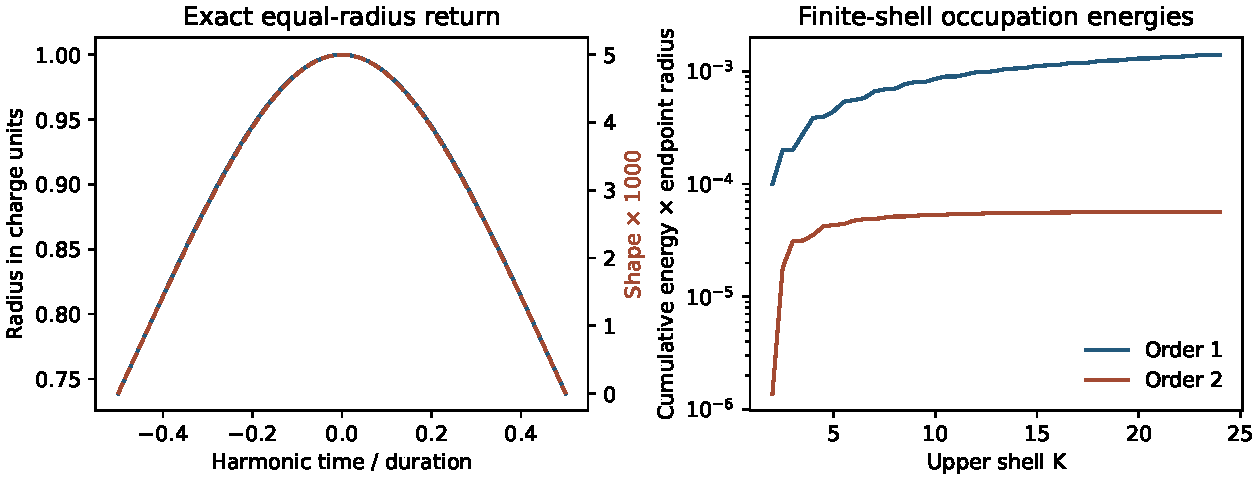
\includegraphics[width=\linewidth]{figures/history.pdf}
\caption{Left: charge-normalized radius (solid) and shape (dashed, right axis) of the exact return. Right: cumulative positive occupation energies through the displayed spherical shells. Each term is obtained from the midpoint of its enclosed probability interval.}\label{fig:history}
\end{figure}

\section{A two-index test on compact Nil}\label{sec:06}
A compact quotient of the Heisenberg group provides a case in which central momentum and oscillator number can grow independently. Write the horizontal radius as $a$, the central radius as $c_N$, and $W=a^2c_N$, with $d\tau=W ds$. Take the standard lattice with Euler number $r_N=1,2$, reference volume $(2\pi)^4/r_N$, and brackets $[e_1,e_2]=(c_N/a^2)e_3$. For $r_N=1$ we take spin structures $(0,0,0)$ and $(1/2,0,0)$; for $r_N=2$ we take $(0,0,0)$ and $(0,0,1/2)$. The fixed-charge data and Clifford orientation are those of Paper~08 \cite{paper8}. The oscillator decomposition for compact Heisenberg quotients is standard \cite{ammann}.

Choose an expanding, initially isotropic velocity at $s=0$, $a(0)=c_N(0)=1$, $h_H=0,1$ for the minimal and real Holst cases, and signed $u_0=\pm1/8,\pm3/8$. With $d_H=1+h_H^2$, the fixed flux is $p_\theta=-Q_\Sigma=6V_\Sigma u_0$ and $\kappa^2 W\,d\theta/d\tau=d_Hu_0$. The Hamiltonian constraint gives $H^2=d_Hu_0^2+1/12$, $H>0$. Spatial Ricci eigenvalues $(-t^2,-t^2,t^2)/2$, $t=c_N/a^2$, give $(\log a)''=c_N^4/2$, $(\log c_N)''=-c_N^4/2$. Thus, defining $D_N=\sqrt{H^2+1/4}$,
\begin{equation}
 E=ac_N=e^{2Hs},\quad Y=c_N^{-2}=\cosh(2D_Ns)-(H/D_N)\sinh(2D_Ns),
 \quad A_N=a^2=E^2Y .                                      \label{eq:nilbg}
\end{equation}
Both intervals $[-1/2,0]$ and $[0,3/2]$ are compact and regular. The following proof concerns the massless field. The massive finite-shell sign readout of Paper~08 also needs a common preparation and detector, and is not an input to the double sum.

For nonzero central label $k=r_N|j+\delta_3|$, $\nu=k/(2\pi)$, a paired level $n\ge1$ has the tracefree harmonic-time Weyl Hamiltonian, up to fixed conjugations,
\begin{equation}
 x\sigma_x+z\sigma_z,\qquad x=\sqrt{2\nu n}\,E,\quad z=\nu A_N,
 \quad \Omega=(x^2+z^2)^{1/2}.                              \label{eq:nilham}
\end{equation}
The two central signs together have multiplicity $2k$ in the paired tower. The axial charge reverses a common scalar phase. Energy sign crossings caused by the bounded scalar shift affect only finitely many low modes on these intervals. At central label zero the torus modes have fixed axis since both horizontal lengths coincide; the unpaired lowest central tower is also diagonal. The infinitely many paired levels determine ultraviolet implementability.

\begin{proposition}
On both intervals, for each specified lattice, spin structure, charge and Holst parameter, the instantaneous endpoint evolution is not implementable. The order-one endpoint prescription gives Hilbert--Schmidt off-diagonal parts.
\end{proposition}
\begin{proof}
Let $L_N=\sqrt{k(k+n)}$, $F_N=\sqrt{kn}/(k+n)$, and $\vartheta=\operatorname{atan2}(x,z)$. The background and finitely many derivatives are uniformly bounded, with positive lower bounds on $A_N,E$. Then $\Omega\asymp L_N$, its finite-order derivatives are $O(L_N)$, and
\[
 \vartheta'=2(v_N-H)\frac{xz}{x^2+z^2},\qquad v_N=(\log c_N)',
 \qquad \partial_s^j\vartheta'=O(F_N).
\]
The last assertion follows by factoring the positive coefficients of $x,z$ before differentiating; $xz/(x^2+z^2)\asymp F_N$. In the instantaneous frame the matrix is $\Omega\sigma_z-\vartheta'\sigma_y/2$. The next rotation has magnitude $|\arctan[-\vartheta'/(2\Omega)]|=O(F_N/L_N)$, as do its finite derivatives. Applying integration by parts as in \eqref{eq:ibp} with residual derivative of this angle gives
\[
 |\beta_1|=O(F_N/L_N^2),\qquad
 |\beta_1|^2=O\!\left(\frac{n}{k(k+n)^4}\right).
\]
Summing with multiplicity $2k$ first on $k+n=\ell$ leaves $\sum_{\ell}O(\ell^{-2})$. The positive permitted central labels here are integer lattices or their parity subsequences. Other fixed finite multiplicity factors do not affect convergence.

For the converse, one endpoint of each interval is $s=0$, where $v_N=H$ and the instantaneous and first-order axes coincide. At the other end $v_N-H\ne0$ since $v_N'=-c_N^4/2<0$. On $1\le n/k\le2$ the nonzero mismatch angle, divided by two, has magnitude $|\vartheta'|/(4\Omega)+O(k^{-3})\ge c/k$ for large $k$. The first-order transport error is $O(k^{-2})$ there. With only one mismatched end its oscillatory phase cannot cancel this leading mixing. A shell with central label $k$ contains order $k$ such oscillator labels and order $k$ copies at each, so its instantaneous squared sum is bounded below by a positive constant. Both parity subsequences have positive density. This proves divergence for both directions.
\end{proof}
As a check, for $u_0=3/8$, $h_H=0$, $[0,1.5]$, one copy at $k=n=1$ gives probabilities $0.0279303$ and $0.0169350$. At $k=n=128$ the corresponding direct values are $1.8407\times10^{-7}$ and $4.8238\times10^{-11}$. These sample probabilities are numerical diagnostics of Eq.~\eqref{eq:nilham}; the double-series test uses uniform inequalities over the unbounded tower.

\section{Discussion}\label{sec:07}
On the spherical history the two round boundary metrics determine the same instantaneous spectral subspaces. The failure of their implementability under propagation depends on the first time derivative of shape. Including this derivative at the endpoints removes the leading mismatch. The next surviving boundary term has nonzero coefficient on a band of magnetic labels; oscillatory phases suppress some individual modes but leave a positive band average. This explains why the same first-order prescription yields finite number and divergent energy. The compact Nil example exhibits a different lower-bound mechanism: one endpoint is shear-free, so no two-end interference has to be averaged.

Both examples start with a prescribed external field, geometry and family of particle definitions. Their conclusions give concrete criteria for finite endpoint observables on these backgrounds. Extending the energy threshold to massive fields or to general Nil histories requires new high-mode estimates. A local stress tensor would additionally involve state regularity and covariant subtraction. On a generic anisotropic three-manifold the number of independent labels and the spectral multiplicities may differ; these enter explicitly in both proofs.

\section*{Availability}
The accompanying repository contains the source, Japanese companion and reproducibility supplement.
\section*{Acknowledgments}
The author acknowledges Claude Opus 5.5, Gemini 4 Neon and GPT Astra 6.2 for assistance during preparation of the manuscript in November 2026, including symbolic derivations, implementation, Japanese--English exposition and deterministic figure-generation code. The calculations and figures are reproducible from the supplied mathematical definitions and data. The author takes responsibility for the content and remaining errors.

This work was developed within the informal collaborative project \textbf{DPPU} (\textbf{D}onut-like topology, \textbf{P}lanck-scale compactness, \textbf{P}recession dynamics, \textbf{U}niverse).
\appendix
\section{Certified low shells and the infinite tail}\label{app:A}
To evaluate Table~\ref{tab:numeric} we split harmonic time into 64 cells of width $\delta=D/64$. In a cell's rescaled real variable $t$, write the Taylor series for one column of the propagator. The coefficients obey
\[
 (m+1)Y_{m+1}=-i\delta\sum_{j=0}^m H_jY_{m-j}.
\]
We retain degrees 0 through 31, reconstructing the other column by the $SU(2)$ conjugation relation. For complex time within radius $\rho=1/5$ of a real basepoint, $\lvert v\rvert\le v_* = z/\cos(2z\rho)$ since $\lvert\cosh(x+iy)\rvert\ge|\cos y|$ in this strip. Similarly $\lvert v^2/u\rvert\le v_*^2\cosh(2y(D/2+\rho))/y$. Let $H_*$ be twice the sum of these bounds; the complex propagator norm is at most $\exp(\rho kH_*)$. The bound on the tail of the series on one step is therefore
\[
 \varepsilon_k=e^{\rho kH_*}(\delta/\rho)^{32}/(1-\delta/\rho).
\]
Real evolution is unitary, so replacing one exact step at a time in the matrix product gives total truncation error at most $(1+\varepsilon_k)^{64}-1$. Apply this to the projected amplitudes before squaring. All arithmetic, elementary functions and endpoint rotations in the enclosure use 180-bit real or complex balls (Arb via python-flint). The positive root for $D$ is isolated by bisection and an interval sign test. The fast real-time DOP853 integrations on representative rays provide a separate check of the spin and derivative signs.

For $k>K=24$, partition the positive half-time interval into 96 pieces and $0\le\mu\le1$ into 20 pieces, taking $0\le\epsilon\le1/K$ as one full interval. Parity and the explicit factors in \eqref{eq:jets} cover the other half and negative labels. For the normalized coefficients in that equation, the interval Taylor derivatives bound $|V_f|$ by $B_*=0.012979$ and
\[
 |J/\omega_2|_f+\tfrac12\int_i^f\Bigl(|(J/\omega_2)'|+
                  K^{-2}|J^2/\omega_2|\Bigr)ds\le C_*=0.084778.
\]
Equation~\eqref{eq:ibp} and the endpoint basis rotations imply $|\beta_2|\le |p|C_*/k^3$, $|\beta_1|\le |p|(B_*/k^2+C_*/k^3)$. To see the second estimate, insert the order-two endpoint bases into the order-one transition. The difference of each endpoint unitary from the identity has norm at most $|\alpha_2|/2$; the error is the sum of the initial and final bounds. For the full magnetic grid,
\[
 \sum_{M=-k}^k p^2=\frac{4k^4-5k^2+1}{15k^3}\le4k/15 .
\]
This identity follows by subtracting the fourth-power sum divided by $k^4$ from the square sum divided by $k^2$ on the unit-spaced grid; it includes both half-integral and integral $k$. Multiplication by two chiralities and $2k$ spectators and comparison of the half-integer shell sum with twice the integral gives
\begin{align}
 S_{1,>K}&\le\frac{32}{15}\left[\frac{B_*^2}{K}
             +\frac{B_*C_*}{K^2}+\frac{C_*^2}{3K^3}\right],&
 S_{2,>K}&\le\frac{32C_*^2}{45K^3},\nonumber\\
 q_e\Delta E_{2,>K}&\le\frac{64 C_*^2}{15K^2}.
\end{align}
For the displayed bounds we used the unrounded interval constants. The supplied code generates the mode labels and the high-mode enclosure independently of the saved tables. A second routine checks the tables by reassembling all 551 mode weights and comparing them with the finite sums.

\section{A third-order comparison}\label{app:B}
For $\chi=+1$ set $\omega_0=\lambda$, $T_1=F$. Defining successive rotation angles by $\tan\alpha_m=p\epsilon^m T_m$, the iteration is
\[
 d_m=1+p^2\epsilon^{2m}T_m^2,\qquad
 \omega_m=\omega_{m-1}\sqrt{d_m},\quad J_m=\frac{T_m'}{2d_m},\quad
 T_{m+1}=(-1)^m\,J_m/\omega_m .
\]
The sign alternates as the rotations use the $x$ and $y$ axes in turn. The residual is $h_m=p\epsilon^mJ_m$. Positivity of $\omega_m$ on the compact parameter box gives $|\beta_3|\le C_3|p|/k^4$ by the same integration by parts. This faster ultraviolet falloff does not order the total occupations. Using $K=32$ (991 positive magnetic pairs) in both the order-two and order-three calculation, including the corresponding unbounded tails, gives
\[
 2.02282\le S_3/S_2\le2.02964,\qquad
 1.25775\le\Delta E_3/\Delta E_2\le1.31281 .
\]
For example, the $k=2$ one-direction shell count changes from
$3.19231\times10^{-6}$ to $8.07695\times10^{-6}$. At order three it already accounts for more than $98\%$ of the total. The archive contains the independent $K=32$ computation with 200-bit arithmetic, 40 cells per time half and degree 37. Comparison at successive orders on one history gives no monotonicity principle or convergence prescription for an infinite sequence of vacua.

\begin{thebibliography}{99}\small
\bibitem{avron} J. E. Avron, S. Bachmann, G. M. Graf and I. Klich. Fredholm determinants and the statistics of charge transport. Commun. Math. Phys. 280 (2008), 807--829. Proposition 5. \url{https://arxiv.org/abs/0705.0099}.
\bibitem{gibbons} G. W. Gibbons. Spectral asymmetry and quantum field theory in curved spacetime. Annals of Physics 125 (1980), 98--116. \url{https://doi.org/10.1016/0003-4916(80)90120-7}.
\bibitem{vardanyan} T. Vardanyan. Matter-antimatter asymmetry in a rotating universe: Dirac spinors in axisymmetric Bianchi IX cosmology. Phys. Rev. D 113 (2026), 023536. \url{https://arxiv.org/abs/2507.12164}.
\bibitem{cortez} J. Cortez, B. Elizaga Navascu\'es, M. Mart\'in-Benito, G. A. Mena Marug\'an and J. M. Velhinho. Unitary evolution and uniqueness of the Fock representation of Dirac fields in cosmological spacetimes (2015). \url{https://arxiv.org/abs/1509.09086}.
\bibitem{navascues} B. Elizaga Navascu\'es, G. A. Mena Marug\'an and S. Prado. Fock quantization of the Dirac field in hybrid quantum cosmology: Relation with adiabatic states (2019). \url{https://arxiv.org/abs/1910.01346}.
\bibitem{hollands} S. Hollands. The Hadamard condition for Dirac fields and adiabatic states on Robertson--Walker spacetimes. Commun. Math. Phys. 216 (2001), 635--661. \url{https://arxiv.org/abs/gr-qc/9906076}.
\bibitem{ammann} B. Ammann and C. B\"ar. The Dirac operator on nilmanifolds and collapsing circle bundles. Ann. Global Anal. Geom. 16 (1998), 221--253. \url{https://arxiv.org/abs/math/9801091}.
\bibitem{paper8} Muacca. Reading the sign of a Nieh--Yan charge on compact spin three-manifolds. v1 (2026). \href{https://doi.org/10.5281/zenodo.24434717}{doi:10.5281/zenodo.24434717}.
\bibitem{paper10} Muacca. Multiplicity of Real Lorentzian Histories Between Two Round Three-Spheres in Biaxial Bianchi IX with Fixed Scalar Charge. v1 (2026). \href{https://doi.org/10.5281/zenodo.24435081}{doi:10.5281/zenodo.24435081}.
\end{thebibliography}
\end{document}
